\chapter{Preliminaries}

\label{chapter:preliminaries}
\section{Homogenous coordinate system}

In projective geometry, the homogenous coordinate system is used the same way as Cartesian coordinates in Euclidean geometry.
To transform a point $x=(u, v)^\top$ from cartesian coordinates to homogenous, simply append $1$ as the third coordinate: $x=(u, v, 1)^\top$.
Homogenous coordinates are used to simplify the 2D transformation operations: 


\begin{equation}
    \vec{m}_1 = 
    \pmb{\mathsf{S}} \pmb{\mathsf{R}}
    \vec{m}_0
    + \vec{t} ;
\end{equation}

\begin{equation}
    \pmb{\mathsf{S}} = \begin{bmatrix} s_x & 0 \\ 0 & s_y \end{bmatrix}, \pmb{\mathsf{R}} = \begin{bmatrix} \cos(\theta) & -\sin(\theta) \\ \sin(\theta) & \cos(\theta) \end{bmatrix}, \vec{t} = \begin{bmatrix} t_x \\ t_y \end{bmatrix} ;
\end{equation}

where $m_0$ is an original point,
$m_1$ is a transformed point,
$\pmb{\mathsf{S}}$ is a scale matrix,
$\pmb{\mathsf{R}}$ is a rotationa matrix and 
$\vec{t}$ is a translation vector.

For an object's transformation, a sequence of matrix multiplications is required. 
However, this is not the case with translation - an addition operation is needed for that. 
Here are these operation in projective geometry:

\begin{equation}
    \begin{bmatrix} \vec{m}_1 \\ 1 \end{bmatrix} = 
    \pmb{\mathsf{S}}_H \pmb{\mathsf{R}}_H \pmb{\mathsf{T}}_H
    \begin{bmatrix} \vec{m}_0 \\ 1 \end{bmatrix} ;
\end{equation}
\begin{equation}
    \pmb{\mathsf{S}}_H = \begin{bmatrix} s_x & 0 & 1\\ 0 & s_y & 1 \\ 0 & 0 & 1\end{bmatrix}, \pmb{\mathsf{R}}_H = \begin{bmatrix} \cos(\theta) & -\sin(\theta) & 0 \\ \sin(\theta) & \cos(\theta) & 0 \\ 0 & 0 & 1 \end{bmatrix}, \pmb{\mathsf{T}}_H = \begin{bmatrix} 1 & 0 & t_x\\ 0 & 1 & t_y \\ 0 & 0 & 1 \end{bmatrix} ;
\end{equation}
where $\pmb{\mathsf{S}}_H, \pmb{\mathsf{R}}_H$ and $\pmb{\mathsf{T}}_H$ are homogenous transformation matrices.

So in the homogenous coordinate system, all 2D transformations can be combined and expressed as matrix multiplications.

\subsection{Vanishing point}
\begin{figure}[h]
    \centering
    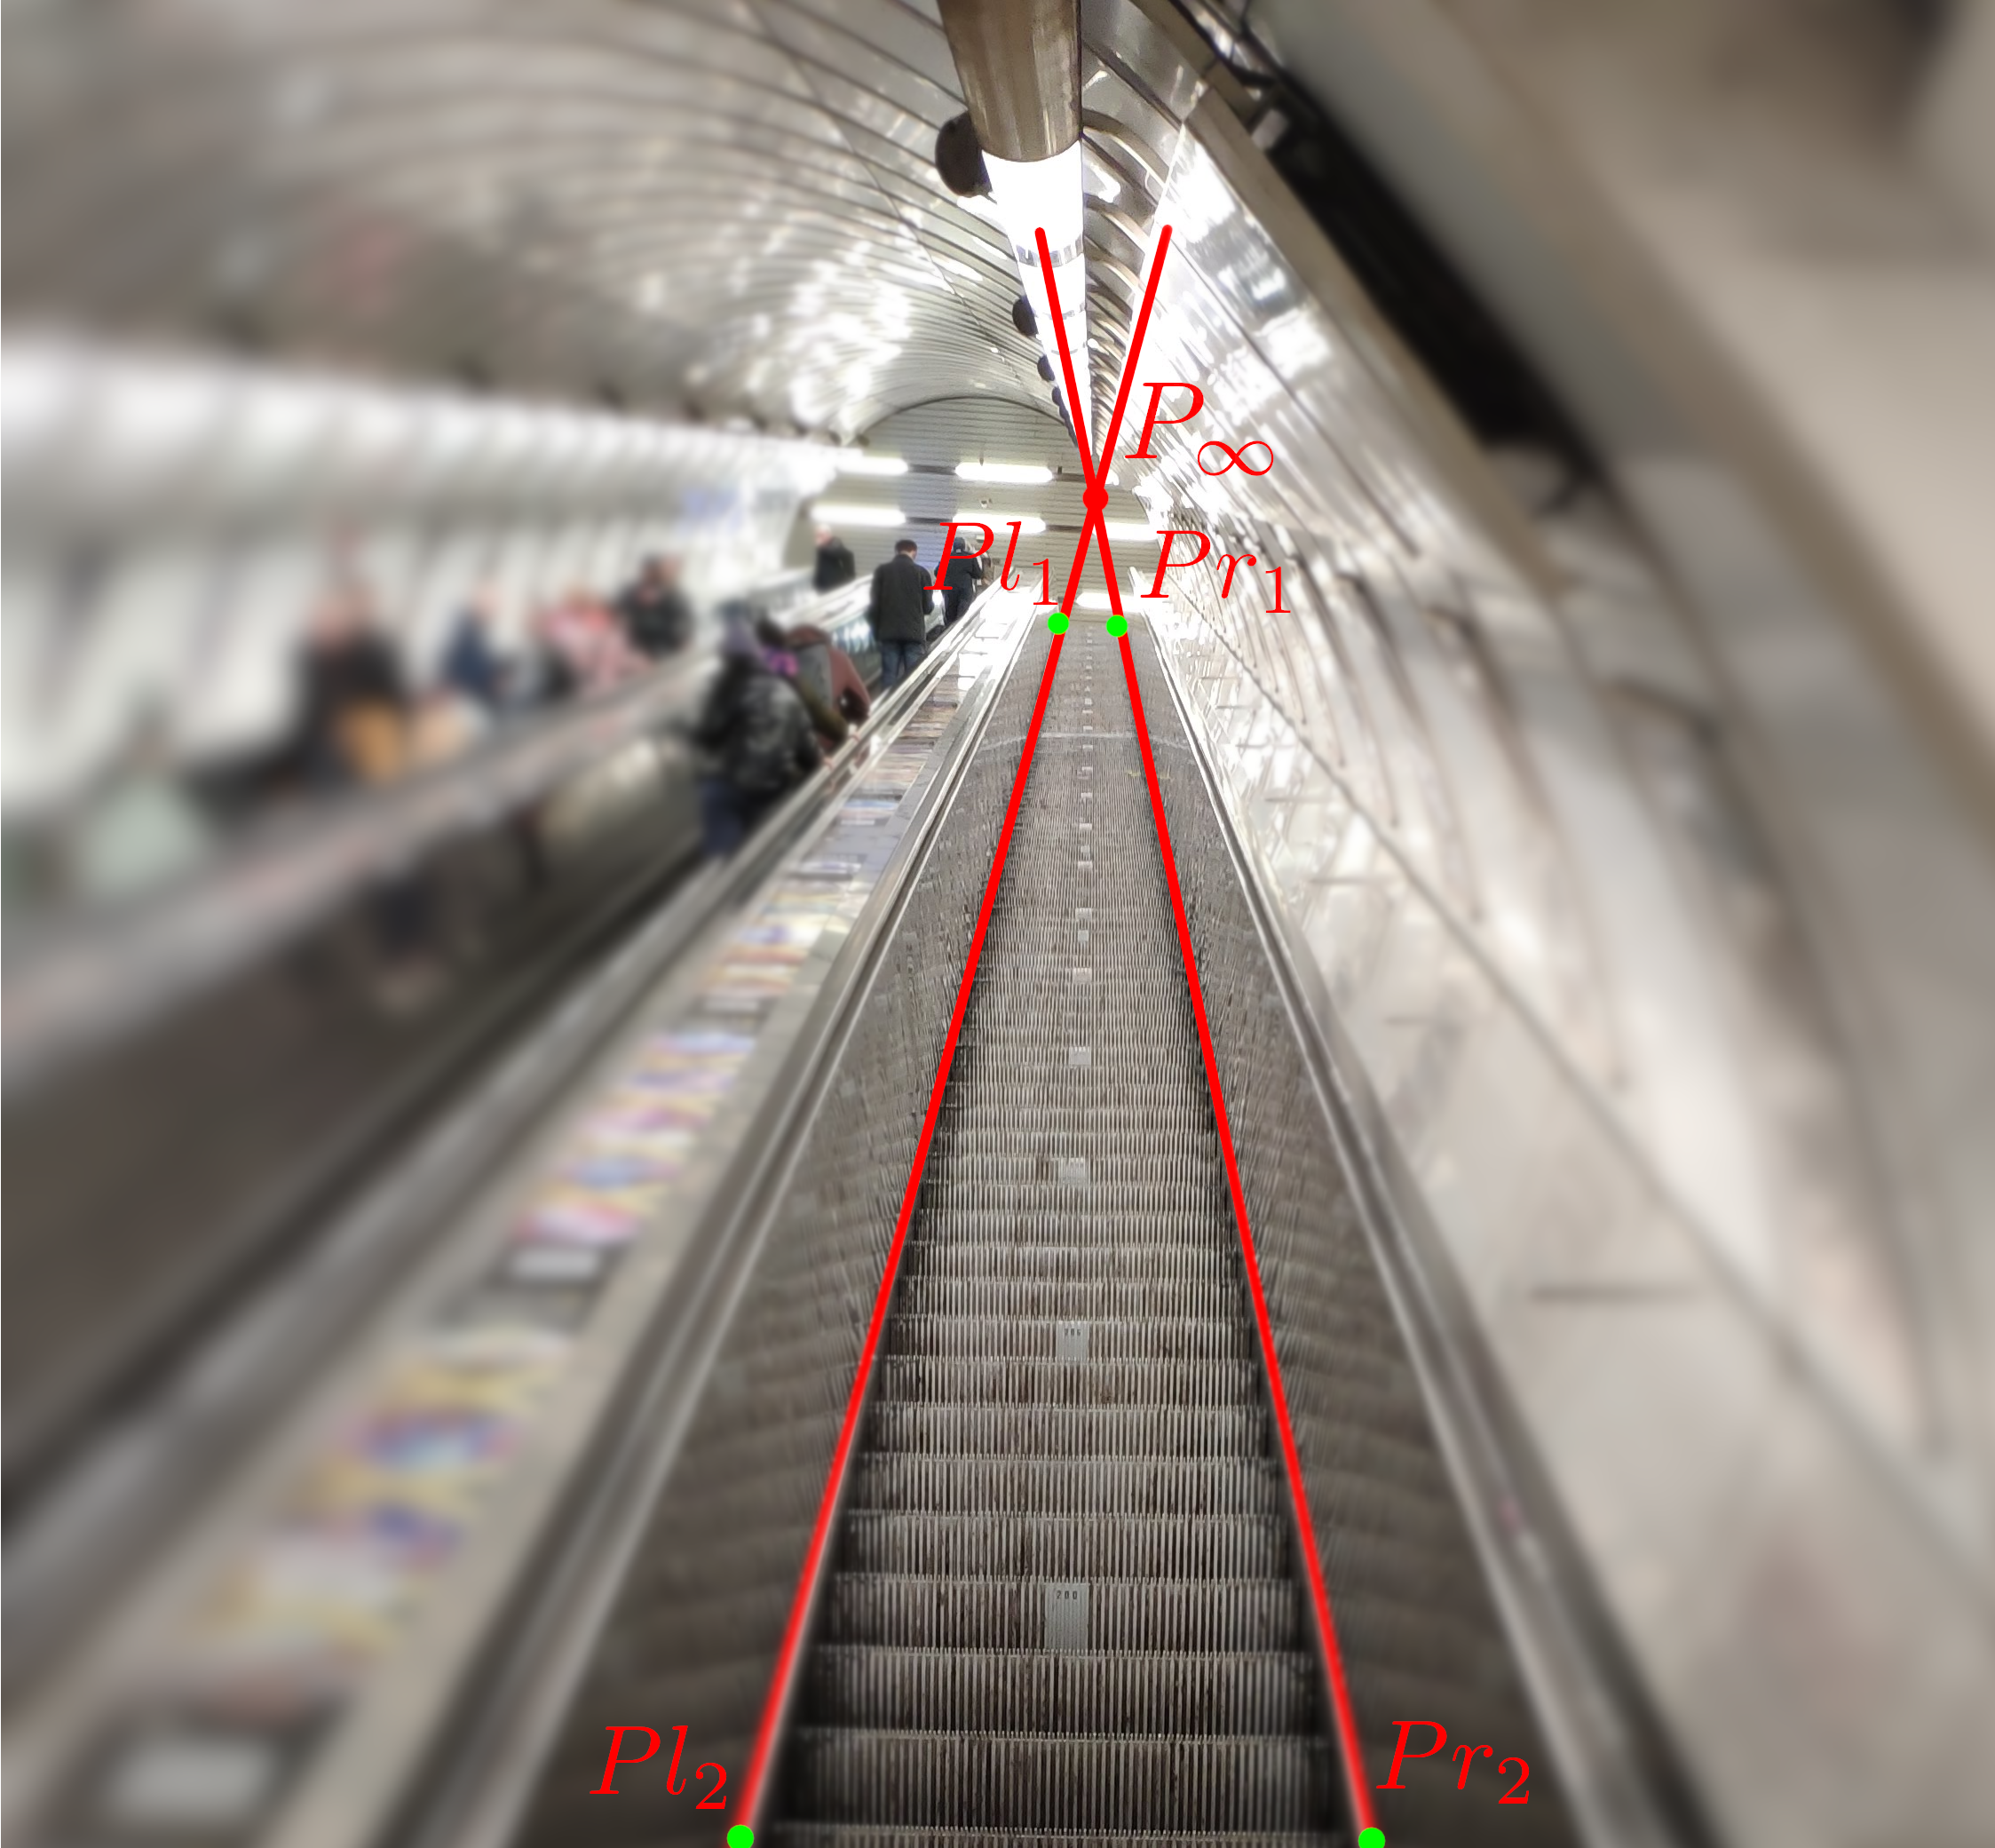
\includegraphics[width=0.75\textwidth]{graphics/parallel_intersection.png}
    \caption{Parallel lines intersection}
    \label{fig:intersection_parallel}
\end{figure}

\begin{figure}[h]
    \centering
    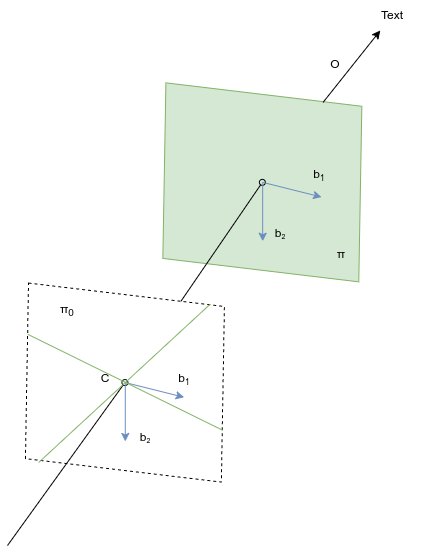
\includegraphics[width=.5\textwidth]{graphics/homogenous.png}
    \caption{Scheme of homogenous coordinates}
    \label{fig:homogenous}
\end{figure}

In Euclidian geometry, parallel lines are the lines that have no intersection point. 
In projective geometry, parallel lines intersect at a point $x$ at infinity. 

In the image \autoref{fig:intersection_parallel} let $\vec{l}_r = Pr_1 \cap Pr_2 $ and $\vec{l}_l = Pl_1 \cap Pl_2$. 
In the 3D world, lines $\vec{l}_l \parallel \vec{l}_r$, but after projection on the image plane $\pi$, in this case it is seen the intersecting point $P_{\infty}$
In general cases, such a point can be computed as a cross product of two parallel lines. 

Both line and point in a homogenous coordinates are expressed as vectors of three numbers: a homogenous point $\vec{m} = (x, y, z)^\top$ is $\vec{m} = (\frac{x}{z}, \frac{y}{z})^\top$, and a line $\vec{l} = (a, b, c)^\top$, where $a, b, c$ are parameters of a line equation $ax + by + c = 0$. 
In general case, point at infinity is called an \textit{ideal point} and it is not seen on the image, it's coordinates can be expressed as $\vec{m}_{\infty} = (u, v, 0)^\top, \{u, v\} \neq 0$.
Same about line - such line is called \textit{ideal line} and it's coordinates are $\vec{l} = (0, 0, c)^\top, c \neq 0$. In algebraic representation, both ideal point and line are at the plane $\pi_0$ (\autoref{fig:homogenous}, green lines).

A vanishing point is an image of the point at infinity.
All world (4D) parallel lines share the same image vanishing point. On a \autoref{fig:intersection_parallel} a $P_{\infty}$ is an image of two parallel lines' intersection point (which is a point at infinity), so it is also a vanishing point.

\section{Pinhole camera model}
A pinhole camera - or a canonical perspective camera model - is a model of a simple camera without any optics.
The first example is a camera obscura - a dark room with a small hole through which the image from outside is projected on the opposite wall. 
This model can be used to express camera geometry with a field of view angles less than $180^{\circ}$.

\subsection{Camera coordinate system}
\begin{figure}[h]
    \centering
    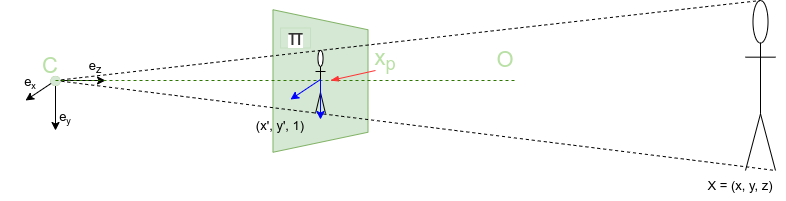
\includegraphics[width=1\textwidth]{graphics/td_scene.png}
    \caption{The pinhole camera model working scheme}
    \label{fig:td_scene_3d}
\end{figure}

\begin{figure}[h]
    \centering
    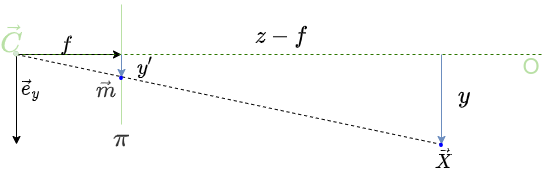
\includegraphics[width=0.9\textwidth]{graphics/td_scene_yz.png}
    \caption{The pinhole camera model, y-z plane}
    \label{fig:td_scene_yz}
\end{figure}

\begin{figure}[h]
    \centering
    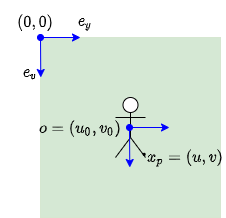
\includegraphics[width=.4\textwidth]{graphics/td_scene_xy.png}
    \caption{The pinhole camera model, x-y plane}
    \label{fig:td_scene_xy}
\end{figure}

In the physical implementation of the Obscure camera, the projective plane is on the opposite side from the Projection centre (or Camera centre $\vec{C}$ in the pinhole camera model), and the image is reversed and mirrored. However, in most computer vision literature, authors assume that it is on the same side as an object (see \autoref{fig:td_scene_3d}).
In \autoref{fig:td_scene_3d} we are looking through a camera with camera center $C$ in a coordinate system with origin at $\vec{C}$ and basis vectors $(\vec{e}_x, \vec{e}_y, \vec{e}_z)$ on a human. 
Each point $\vec{X} = (x, y, z)^\top$ in a world coordinate system has it's projection $\vec{m} = (u, v)^\top$ on a plane $\pi$ which is located on a distance 1 from a camera center (\autoref{fig:td_scene_yz}). 
Optical axis $\vec{O}$ is a ray perpendicular to plane $\pi$, and on the image the point $ \vec{O} \cap \pi = \vec{o}$ is a center of the image, see \autoref{fig:td_scene_xy}.

\subsection{Camera calibration matrix}
\begin{figure}[h]
    \centering
    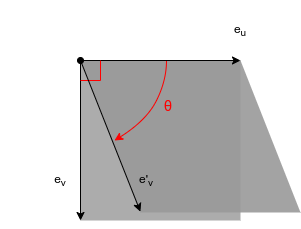
\includegraphics[width=.6\textwidth]{graphics/pixel.png}
    \caption{Scheme of pixel, changing the image (inner) reference frame}
    \label{fig:Kframes}
\end{figure}
Camera calibration matrix - a matrix that includes camera \textit{intrinsic} parameters - pixel size ($e_u$ and $e_v$) and pixel skew angle ($\theta$), as on \autoref{fig:Kframes}, pixel aspect ratio $\bf{a}$ and principle point coordinates $\vec{o} = (u_0, v_0)$ \autoref{fig:td_scene_xy}.
\begin{equation}
    \pmb{\mathsf{K}} = \begin{bmatrix}
        af & -a f \cot(\theta) & u_0 \\
        0 & \frac{f}{\sin(\theta)} & v_0 \\
        0 & 0 & 1 \\
    \end{bmatrix} 
    \textrm{ units: } [f]=px, [u_0]=px, [v_0]=px, [a]=1;
\end{equation}


Where $f$ is a focal length used to convert world length ratios to pixels.

In the modern world, every digital camera has a calibration matrix with a square pixel, so in most cases, the camera matrix looks like this:

\begin{equation}
    \label{eq:kmat}
    \pmb{\mathsf{K}} = \begin{bmatrix}
        f_x & 0 & u_0 \\
        0 & f_y & v_0 \\
        0 & 0 & 1 \\
    \end{bmatrix};
\end{equation}

\subsection{Projection matrix}

\begin{figure}[h]
    \centering
    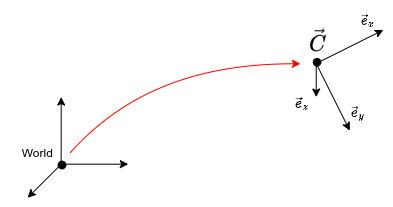
\includegraphics[width=.5\textwidth]{graphics/frames.png}
    \caption{Changing the world (outer) reference frame}
    \label{fig:frames}
\end{figure}

To translate a point from a world coordinate frame to an image coordinate frame, the Image projection matrix $\pmb{\mathsf{P}}$ is used. 
The canonical projection matrix $\pmb{\mathsf{P}}_0$ assumes that the camera is in the world coordinate centre and that the calibration matrix $\pmb{\mathsf{K}} = \pmb{\mathsf{I}}$
\begin{equation}
\pmb{\mathsf{P}}_0 = \begin{bmatrix} \pmb{\mathsf{I}} & | & \vec{0} \end{bmatrix} = 
    \begin{bmatrix}
    1 & 0 & 0 & 0 \\
    0 & 1 & 0 & 0 \\
    0 & 0 & 1 & 0 \\
    \end{bmatrix};
\end{equation}

However, this case is degenerate. 
As far as each camera is different, the canonical projection matrix is never used. Instead, image projection matrix $\pmb{\mathsf{P}}$ is used, with applied calibration matrix $\pmb{\mathsf{K}}$ to transform canonical $\pmb{\mathsf{P}}_0$ to perspective $\pmb{\mathsf{P}}$:

\begin{equation}
\pmb{\mathsf{P}} = \pmb{\mathsf{K}} \begin{bmatrix} \pmb{\mathsf{I}} & | & \vec{0} \end{bmatrix} = 
    \begin{bmatrix} 
    f_x & 0 & u_0 & 0 \\
    0 & f_y & v_0 & 0 \\ 
    0 & 0 & 1 & 0 \\
    \end{bmatrix}; 
\end{equation}

However, usually, the world coordinate centre is not located at point $\vec{C}$ \autoref{fig:frames}. 
Usually it is rotated using a rotation matrix $\pmb{\mathsf{R}}$ and translated on vector $\vec{t}$ where $\pmb{\mathsf{R}}$ is a $3x3$ matrix with $det(\pmb{\mathsf{R}}) = 1$ and $\pmb{\mathsf{R}}^{-1} = \pmb{\mathsf{R}}^\top$. 
So, in the general case:
\begin{equation}
    \pmb{\mathsf{P}} = \pmb{\mathsf{K}} \begin{bmatrix} \pmb{\mathsf{R}} & | & \vec{t} \end{bmatrix} = 
    \pmb{\mathsf{K}} \begin{bmatrix} \pmb{\mathsf{R}} & | & - \pmb{\mathsf{R}} \pmb{\mathsf{C}} \end{bmatrix};
\end{equation}

where $\vec{C}$ is often used as a camera position in a world reference frame. 
So matrix $\bf{P}$ have six intrinsic parameters: three Euler angles and three translation components. 

\subsection{Projection equation}

Image point $\vec{m} = (u, v)\top$ can be obtained from a 3D point $\vec{X}$ using matrix $\bf{P}$:

\begin{equation}
    \label{eq:projection}
    \lambda \begin{bmatrix} 
        u \\ v \\ 1 \end{bmatrix} = \pmb{\mathsf{P}} \begin{bmatrix} x \\ y \\ z \\ 1
    \end{bmatrix};
\end{equation}

\begin{equation}
    \lambda \begin{bmatrix} 
    \vec{m} \\ 1 \end{bmatrix} = \pmb{\mathsf{P}} \begin{bmatrix} \vec{X} \\ 1
\end{bmatrix};
\end{equation}
Where $\lambda \neq 0$

\section{Epipolar geometry}

\subsection{Skew-symmetric 3x3 matrix}
A skew-symmetric or antisymetric matrix is such matrix $[\vec{b}]_{\times}$ that $[\vec{b}]_{\times}^\top = -[\vec{b}]_{\times}$. 
For vector $\vec{b} = (b_1, b_2, b_3)^\top$:
\begin{equation}
    [\vec{b}]_{\times} = \begin{bmatrix}
        0 & -b_3 & b_2 \\ 
        b_3 & 0 & b_1 \\ 
        -b_2 & b_1 & 0 \\ 
    \end{bmatrix};
\end{equation}

This matrix has some essential properties, but the most important in this thesis - it generalizes across a product as matrix multiplication.
\begin{equation}
    \vec{a} \times \vec{b} = [\vec{a}]_{\times} \vec{b};
\end{equation}
Notation is taken from \cite{hartley_zisserman_2004}, p. 581.
\subsection{Epipolar geometry}
\begin{figure}[h]
    \centering
    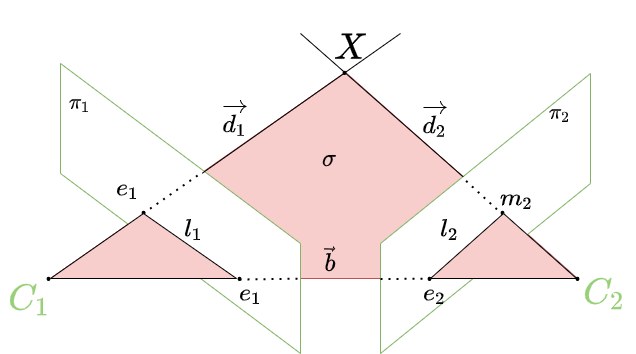
\includegraphics[width=1\textwidth]{graphics/epipolar.png}
    \caption{Epipolar geometry scheme}
    \label{fig:epipolar_std}
\end{figure}

\autoref{fig:epipolar_std} shows a scheme of two cameras with different camera centers $\vec{C}_1$ and $\vec{C}_2$ connected with a base line $\vec{b} = \vec{C}_2 - \vec{C}_1$. 
Both of them are seen as some 3d point $X$. 
This point projections are $\vec{m}_1$ and $\vec{m}_2$ respectivly. 
Points $\vec{C}_1, \vec{C}_2$ and $\vec{X}$ form an \textit{epipolar plane} $\sigma$.
$\sigma \cap \pi_1 = \vec{l}_1$ and $\sigma \cap \pi_2 = \vec{l}_2$ are images of \textit{epipolar lines}. 
Epipolar line $\vec{l}_1$ passes through \textit{epipole} $\vec{e}_1$, where $\lambda [\vec{e}_1 | 1]^\top = \pmb{\mathsf{P}}_2 \vec{C}_1$, same with $\lambda [\vec{e}_2 | 1]^\top = \pmb{\mathsf{P}}_1 \vec{C}_2$.

\subsection{Epipolar constraint}

Having a set of two cameras the relationship between them and constraints on them can be expressed by two new matrices \textit{Essential matrix} $\pmb{\mathsf{E}} \in \mathbb{R}^{3x3}, rank(\pmb{\mathsf{E}}) = 2$, \autoref{eq:E} and \textit{Fundamental matrix} $\pmb{\mathsf{F}} \in \mathbb{R}^{3x3}, rank(\pmb{\mathsf{F}}) = 2$, \autoref{eq:F}
\begin{equation}
    \label{eq:E}
    \pmb{\mathsf{E}} = \pmb{\mathsf{R}}_2 [\vec{C}_2 - \vec{C}_1]_{\times} \pmb{\mathsf{R}}_1^\top = [-\vec{t}_{21}]_{\times} \pmb{\mathsf{R}}_{21} = [\vec{b}]_{\times} \pmb{\mathsf{R}}_{21};
\end{equation}
\begin{equation}
    \label{eq:F}
    \pmb{\mathsf{F}} = \pmb{\mathsf{K}}_2^{-T} \pmb{\mathsf{R}}_2 [\vec{C}_2 - \vec{C}_1]_{\times} \pmb{\mathsf{R}}_1^\top \pmb{\mathsf{K}}_1^{-1} = 
    \pmb{\mathsf{K}}_2^{-T} [-\vec{t}_{21}]_{\times} \pmb{\mathsf{R}}_{21} \pmb{\mathsf{K}}_1^{-1} = 
    \pmb{\mathsf{K}}_2^{-T} \pmb{\mathsf{E}} \pmb{\mathsf{K}}_1^{-1};
\end{equation}
where 
$\pmb{\mathsf{R}}_{21} = \pmb{\mathsf{R}}_2 \pmb{\mathsf{R}}_1^\top$ is a relative camera rotation and 
$\vec{t}_{21} = -\pmb{\mathsf{R}}_2 \vec{b} = \vec{t}_2 - \pmb{\mathsf{R}}_{21}\vec{t}_1$ is a relative camera translation.

An algebraic expression of important properties of matrix $F$:
\begin{equation}
    \label{eq:Fm2}
    \lambda \vec{l}_1 = \pmb{\mathsf{F}}^\top \begin{bmatrix} \vec{m}_2 \\ 1 \end{bmatrix},
\end{equation}
\begin{equation}
    \label{eq:Fm1}
    \lambda \vec{l}_2 = \pmb{\mathsf{F}} \begin{bmatrix} \vec{m}_1 \\ 1 \end{bmatrix},
\end{equation}
\begin{equation}
    \label{eq:fefe}
    \pmb{\mathsf{F}} \begin{bmatrix} \vec{e}_1 \\ 1 \end{bmatrix} = \pmb{\mathsf{F}}^\top \begin{bmatrix} \vec{e}_2 \\ 1 \end{bmatrix} = 0,
\end{equation}
\begin{equation}
    \label{eq:epiconstr}
    \begin{bmatrix} \vec{m}_2 & | & 1 \end{bmatrix} \pmb{\mathsf{F}} \begin{bmatrix} \vec{m}_1 \\ 1 \end{bmatrix} = 0.
\end{equation}
Matrix $\pmb{\mathsf{F}}$ maps points from $\pi_1$ to epipolar lines on $\pi_2$ and vice versa (\autoref{eq:Fm1} and \autoref{eq:Fm2}); epipoles $\vec{e}_1$ and $\vec{e}_2$ are right and left nullspaces basis vectors of $\pmb{\mathsf{F}}$ respectivly (\autoref{eq:fefe}).
Epipolar constraint \autoref{eq:epiconstr} means that a point and it's corespondent line are on a same plane (\autoref{fig:epipolar_std}, plane $\sigma$).

\section{Stereovision}

\begin{figure}[h]
    \centering
    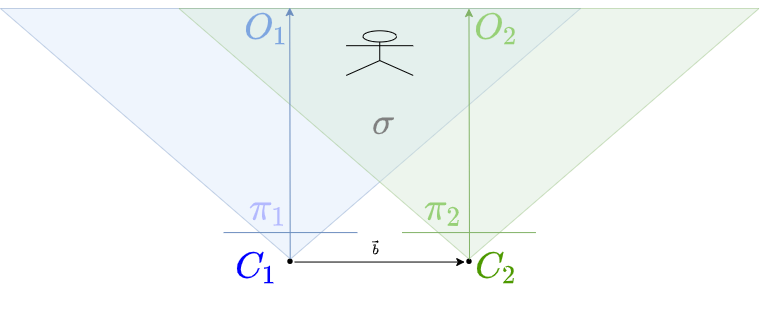
\includegraphics[width=1\textwidth]{graphics/stereopair.png}
    \caption{Scheme of stereovision}
    \label{fig:sch_stereo}
\end{figure}
\begin{figure}[h]
    \centering
    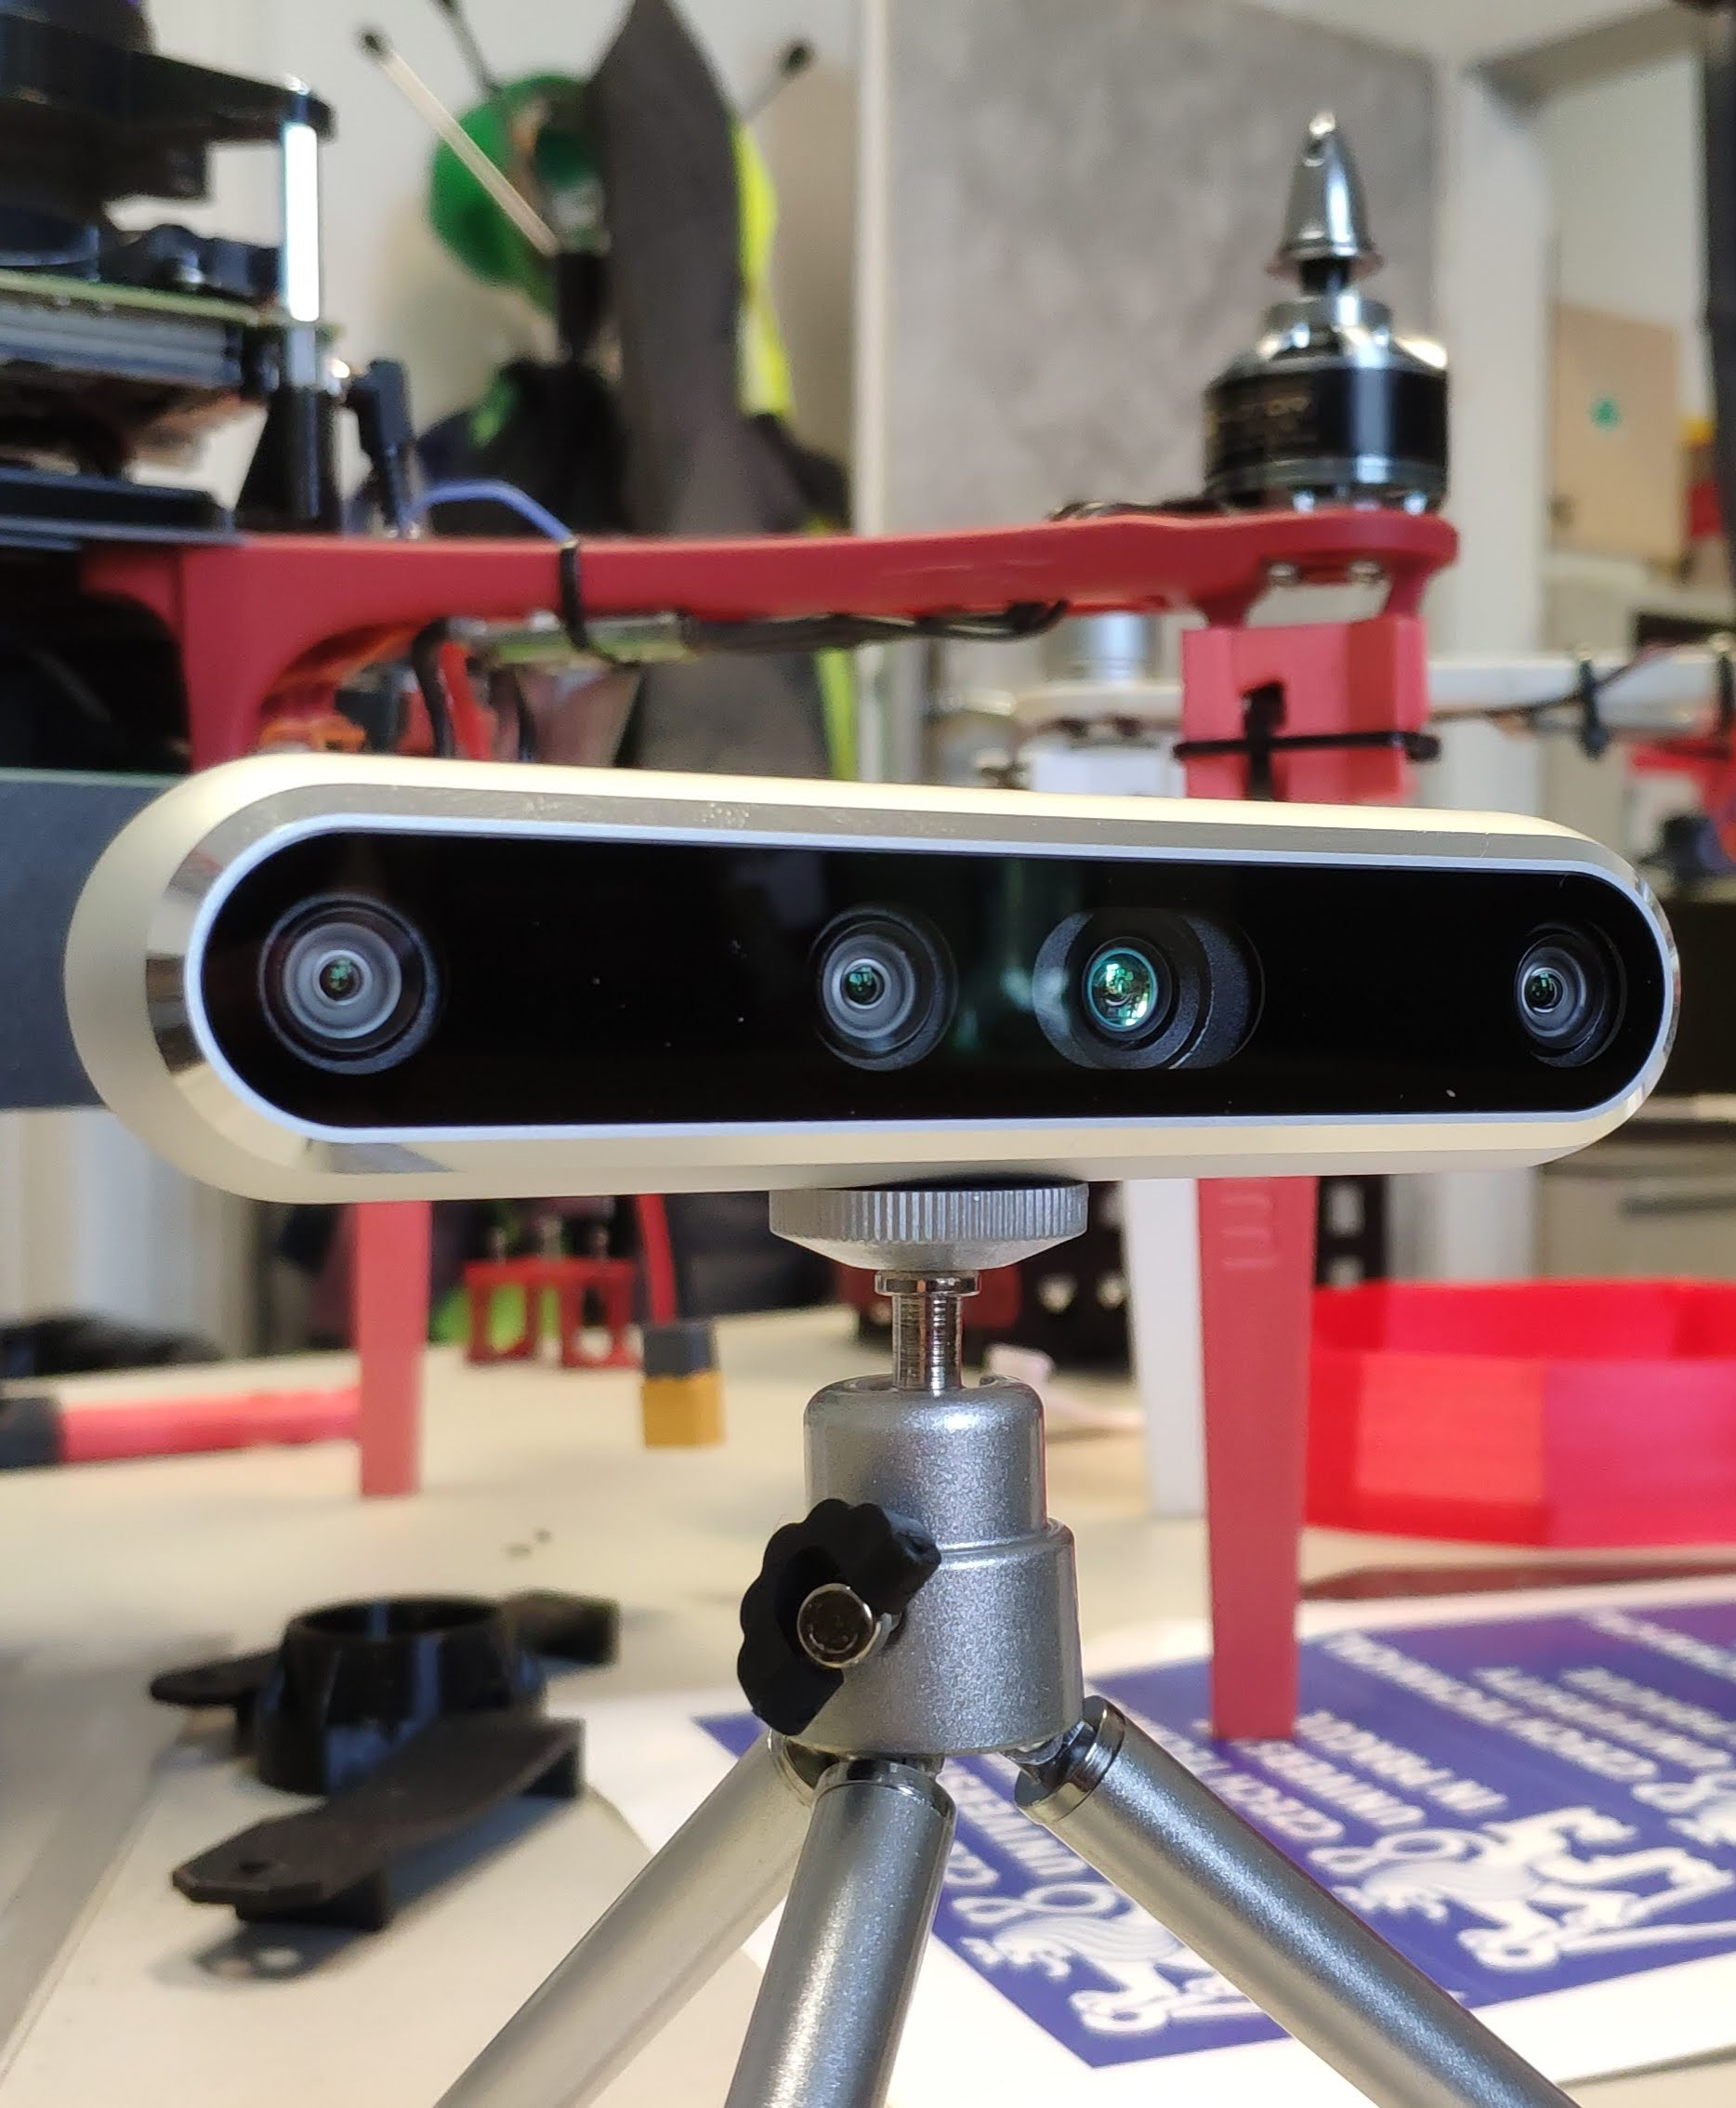
\includegraphics[width=0.5\textwidth]{graphics/stereo_example.jpg}
    \caption{Insustrial stereocamera example, Intel realsense D455}
    \label{fig:stereo_ex}
\end{figure}

\begin{figure}[h]
    \begin{subfigure}[b]{0.31\textwidth}
      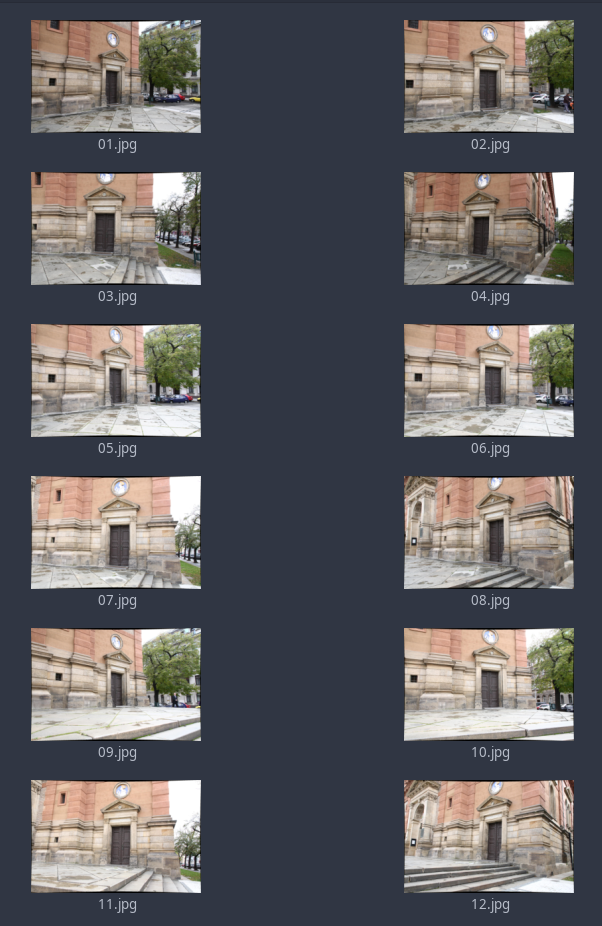
\includegraphics[width=\textwidth]{graphics/input_set.png}
      \caption{Input set of images.}
      \label{fig:pc_input}
    \end{subfigure}
    \hfill
    \begin{subfigure}[b]{0.65\textwidth}
      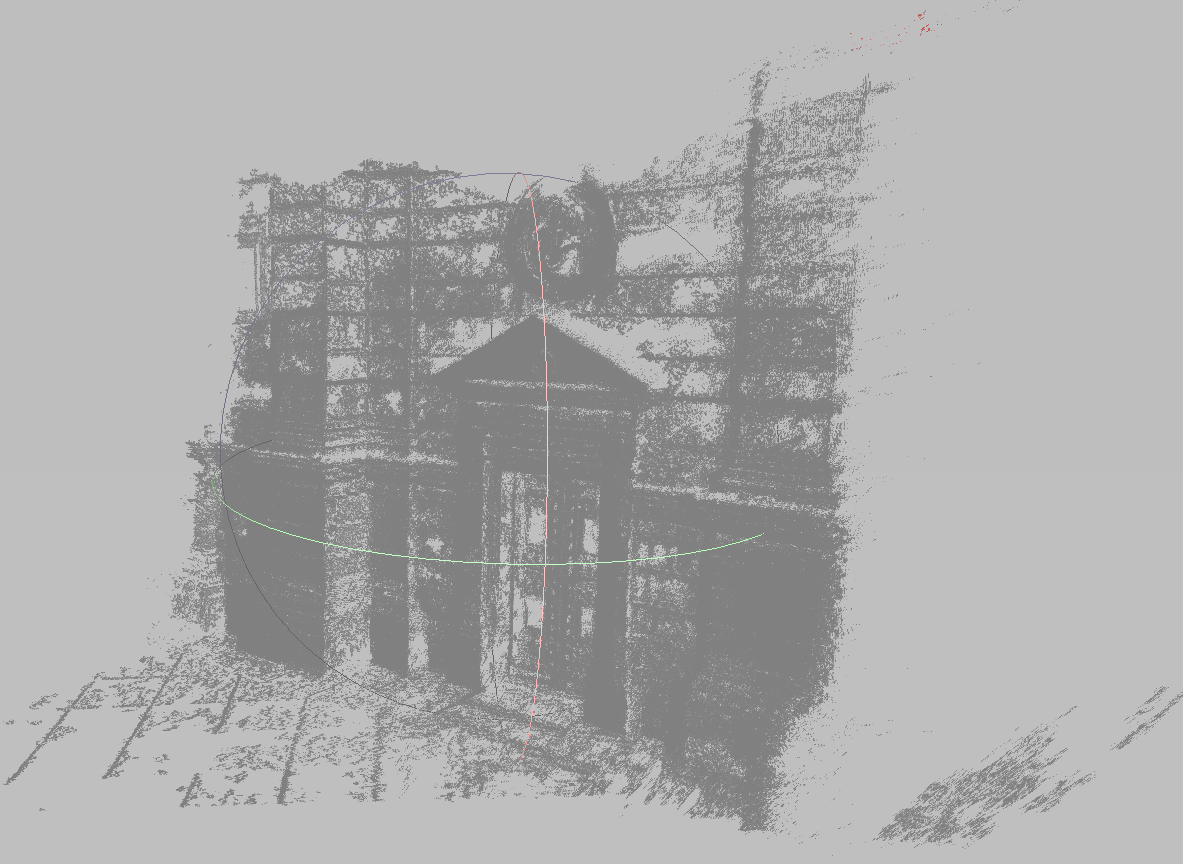
\includegraphics[width=\textwidth]{graphics/reconstructed.png}
      \caption{reconstructed pointcloud.}
      \label{fig:pc_output}
    \end{subfigure}
    \caption{Three dimensional reconstruction from multiple cameras.}
    \label{fig:pc_recons}
\end{figure}

Computer stereo vision is a process of extracting a stereo (depth) image from a planar image or set of images of the same scene. Usually, a stereo camera has two simple cameras located at some distance $\vec{b}$ pointing in the same direction, the same as the human eye (the scheme \autoref{fig:sch_stereo} and an example of a stereo camera \autoref{fig:stereo_ex}). 
Sometimes fusion of multiple cameras and other sensors can be used:
Intel Realsense \autoref{fig:stereo_ex} has two cameras, an IR sensor in case the images have almost no texture and a color sensor. 

\begin{equation}
    \label{eq:e1e2}
    \vec{e}_1 = \vec{e}_2 = \lambda \begin{bmatrix} 1 \\ 0 \\ 0 \end{bmatrix};
\end{equation}
\begin{equation}
    \label{eq:e1m1}
    \lambda \vec{l}_1 = \vec{e}_1 \times \vec{m}_1 = [\vec{e}_1]_\times \begin{bmatrix} \vec{m}_1 \\ 1\end{bmatrix};
\end{equation}
\begin{equation}
    \label{eq:F_simple}
    \pmb{\mathsf{F}} = \lambda [\vec{e}_1]_\times = \lambda \begin{bmatrix}
        0 & 0 & 0 \\
        0 & 0 & -1 \\
        0 & 1 & 0 \\
    \end{bmatrix};
\end{equation}

It is possible to calculate only the non-zero multiple of $\pmb{\mathsf{E}}$ from image correspondences so that the scene can be reconstructed only up to a scale, but knowing the translation vector $\vec{b}$ (\autoref{fig:sch_stereo}), means having a calibrated stereo pair, all distances can be calculated in world coordinates frame.
By removing a rotation between cameras ($\pmb{\mathsf{R}} = \pmb{\mathsf{I}}$), all computations are simplified.

Corresponding epipolar lines lie on same image rows ($\vec{l}_1 = \vec{l}_2$), and intersects at "points at infinity" (\autoref{eq:e1e2}). 
Epipole is a point of intersecting all epipolar lines, so having the intersecting point ($\vec{e}_1$) and image point epipolar line can be calculated (\autoref{eq:e1m1}), therefore considering \autoref{eq:Fm1}, \autoref{eq:e1e2} and \autoref{eq:e1m1} the \autoref{eq:F_simple} is true.

What is more, consider two correspondences $\vec{a}_1 = (u_1, v)^\top$ and $\vec{a}_2 = (u_2, v)^\top $. For a correspondences matcher it is more efficient to have a predefined corelation between features - and knowing the fact that $v$ coordinate is the same (up to some error) is good enough constraint that can accelerate matching (and looking for more features).

It is possible to receive even a dense point cloud as on \autoref{fig:pc_output} with this approach.


\section{Calibration}
\label{sec:prelimin_calibration}
\subsection{Single camera calibration}

\begin{figure}[h]
    \centering
    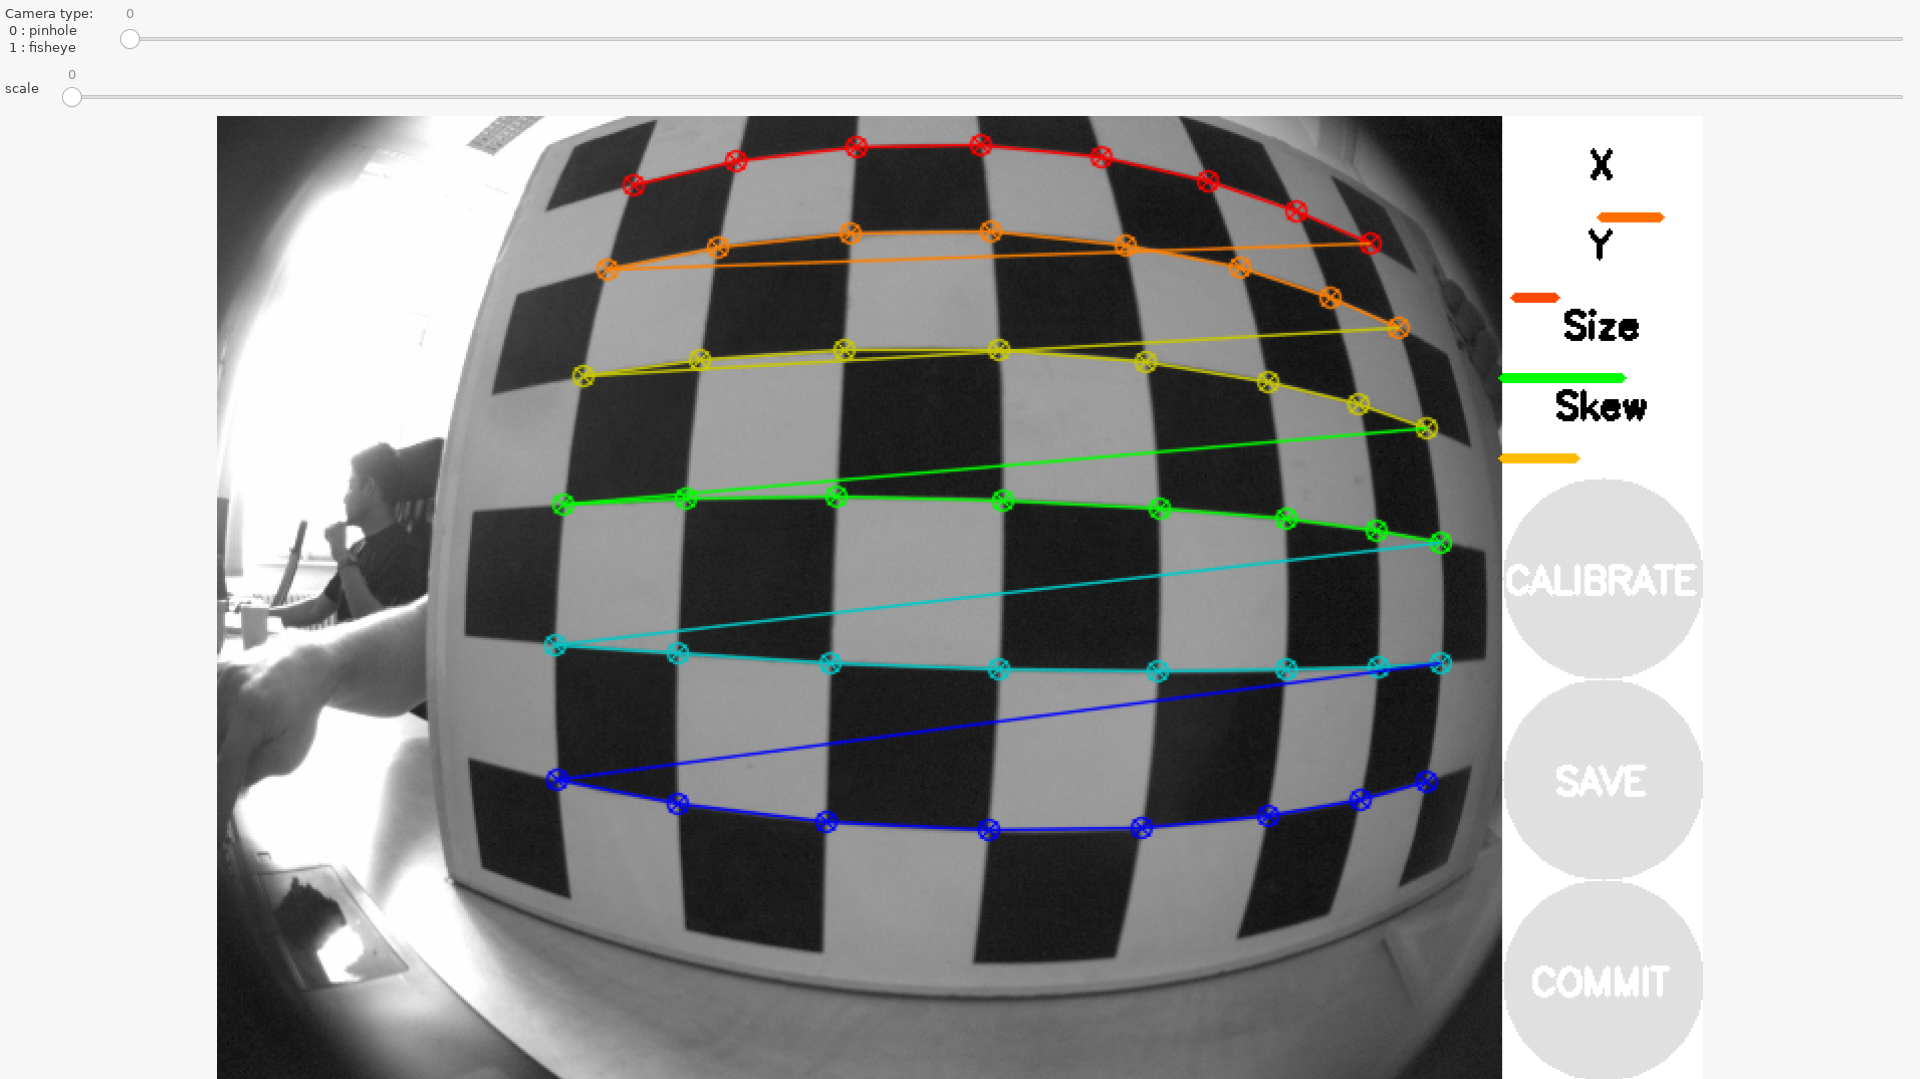
\includegraphics[width=.6\textwidth]{graphics/calibration.png}
    \caption{Calibration process}
    \label{fig:calib}
\end{figure}

\begin{figure}[h]
    \begin{subfigure}[b]{0.45\textwidth}
      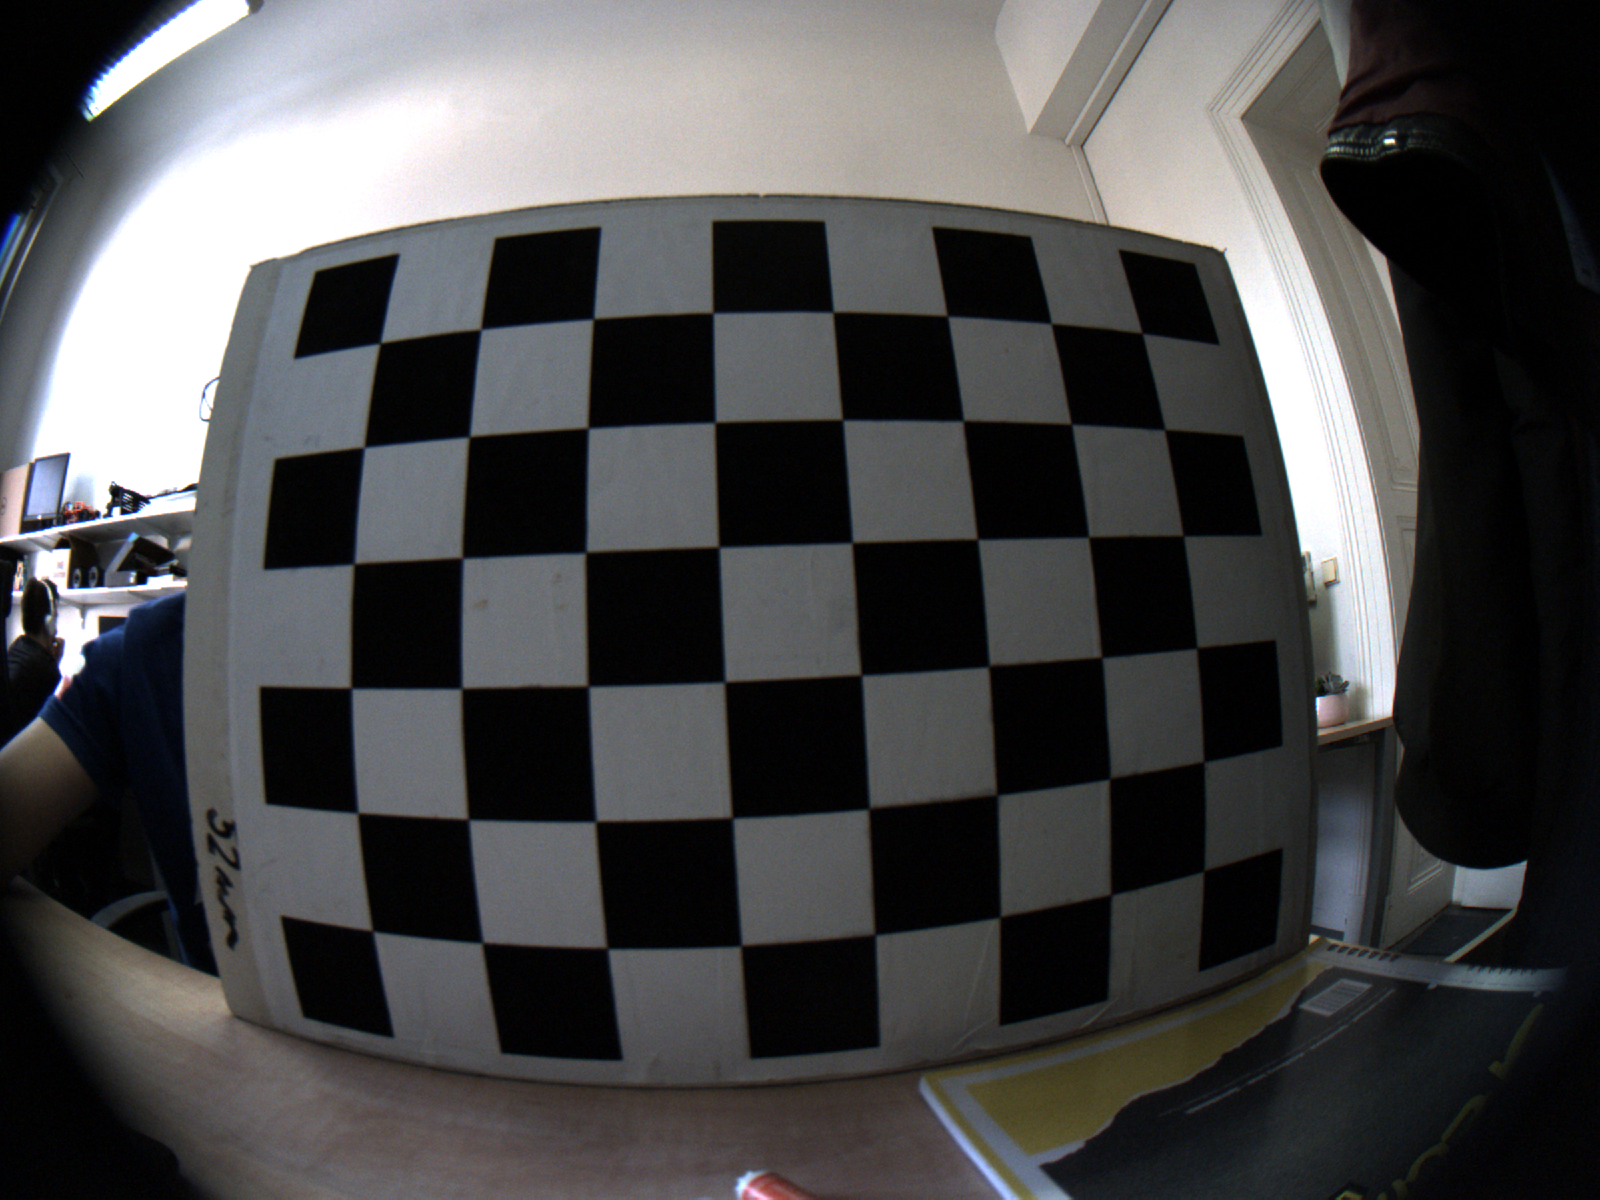
\includegraphics[width=\textwidth]{graphics/chessboard_img.png}
      \caption{Original image with radial distortion.}
      \label{fig:chb1}
    \end{subfigure}
    \hfill
    \begin{subfigure}[b]{0.45\textwidth}
      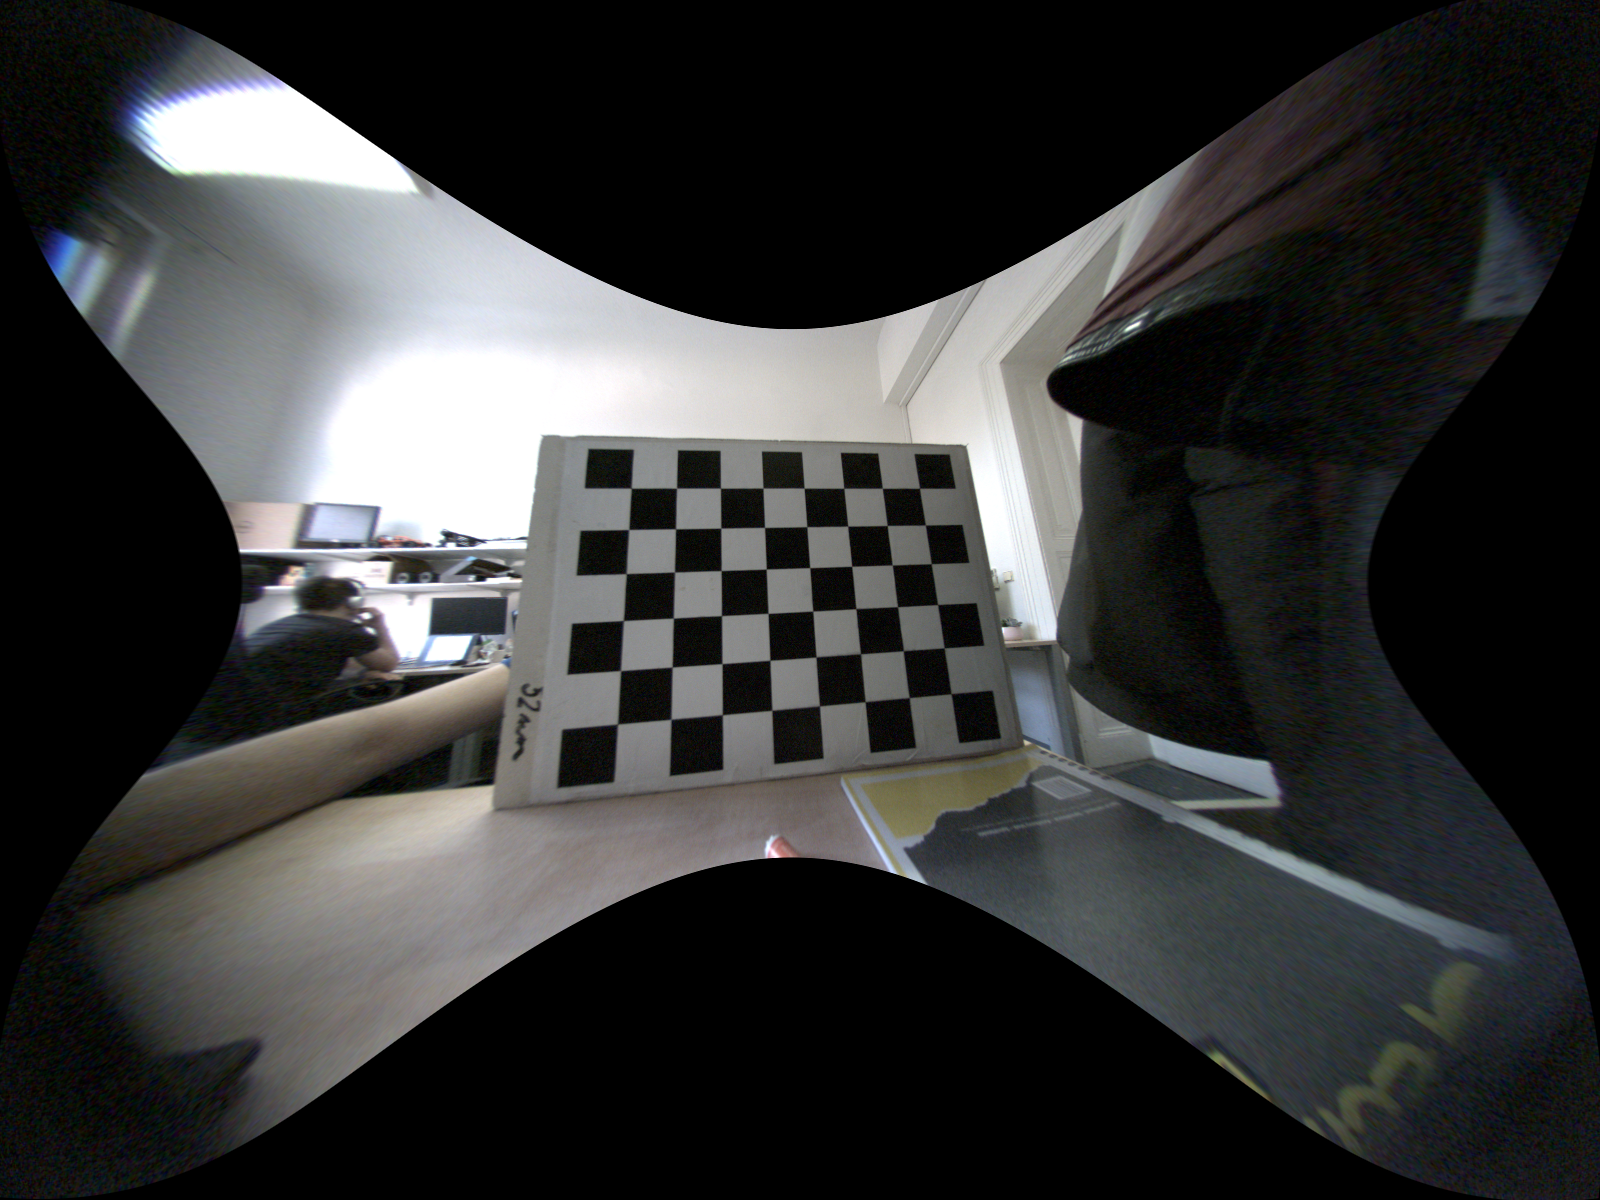
\includegraphics[width=\textwidth]{graphics/chessboard_img_rect.png}
      \caption{Undistorted image with no distortion.}
      \label{fig:chb2}
    \end{subfigure}
    \caption{Camera image before and after the calibration}
    \label{fig:chb}
\end{figure}

Camera calibration - or \textit{Camera resection} process of computing the camera calibration matrix $K$ (\autoref{eq:kmat}).
Usually, it is done with some pattern with predefined parameters, like a chessboard or more advanced boards (ArUco and ChArUco\footnote{\href{https://docs.opencv.org/4.x/df/d4a/tutorial_charuco_detection.html}{Opencv ChArUco and ArUco boards}}).

Camera calibration is necessary for geometry correction (\autoref{fig:chb}), so as a result, parallel lines in 3D are parallel to the image after the undistortion, and the image is unwrapped and projected on a plane.

In a real world lenses has also some distortion (\autoref{fig:chb1}) so to fix that distortion coefficients should be calculated: radial distortion $k_1, k_2, k_3, k_4, k_5, k_6$ and tangential distortion $p_1, p_2$.

From the \autoref{eq:projection}:
\begin{equation}
    \label{eq:dist_start}
    \lambda \begin{bmatrix} 
        u \\ v \\ 1 \end{bmatrix} = \pmb{\mathsf{K}} [\pmb{\mathsf{R}} | \vec{t}] \begin{bmatrix} x \\ y \\ z \\ 1
    \end{bmatrix},
\end{equation}
\begin{equation}
    \label{eq:dist_2}
    \begin{bmatrix} x_c \\ y_c \\ z_c \end{bmatrix}
     = [\pmb{\mathsf{R}} | \vec{t}] \begin{bmatrix} x \\ y \\ z \\ 1
    \end{bmatrix},
\end{equation}
\begin{equation}
    \label{eq:dist_3}
    x'' = \frac{x_c}{z_c} \frac{1 + k_1r^2 + k_2r^4 + k_3r^6}{1 + k_4r^2 + k_5r^4 + k_6r^6} + p_1(r + 2x') + 2p_2\frac{x_c y_c}{z^2_c},
\end{equation}
\begin{equation}
    \label{eq:dist_4}
    y'' = \frac{y_c}{z_c} \frac{1 + k_1r^2 + k_2r^4 + k_3r^6}{1 + k_4r^2 + k_5r^4 + k_6r^6} + 2p_1(\frac{x_c y_c}{z_c^2}) + p_2(r + 2y'),
\end{equation}
where $x' = (\frac{x_c}{z_c})^2$; $y' = (\frac{y_c}{z_c})^2$; $r = x' + y'$. Then undistorted point will be
\begin{equation}
    \label{eq:dist_end}
    \begin{bmatrix} u \\ v \\ 1 \end{bmatrix} = \pmb{\mathsf{K}} \begin{bmatrix} x'' \\ y'' \\ 1 \end{bmatrix}.
\end{equation}

Considering \autoref{eq:kmat}, image of a point $X$ seen through the calibrated camera with projection matrix $P$ will look as in \autoref{eq:dist_start} - \autoref{eq:dist_end}. Firstly, the point is projected on an abstract projection plane (\autoref{eq:dist_2}), then undistorted (\autoref{eq:dist_3}, \autoref{eq:dist_4}) and finally transformed from metric system of abstract projection plane to an image coordinate system (\autoref{eq:dist_end}).

\subsection{Stereopair calibration}

Stereo pair calibration is a process of estimating the essential matrix $E$ for a camera pair, which also can be computed from a relative rotation matrix $\pmb{\mathsf{R}}_{21}$ and a relative translation vector $\vec{t}_{21}$ of a camera pair. 
One approach is to fix one camera pose as world coordinate frame origin and compute a pose of a second camera concerning the first one. 
It can be done with a PnP (Perspective-n-Point) problem solver - estimation of a calibrated camera pose given a set of $n$ 3D points in a world coordinate frame. Minimal required $n=3$. 

Another possible approach is to give an initial guess of a camera pose, and two sets of 3D points from both cameras fix the error by minimisation the transformation between that point sets. This approach is described in \cite{Umeyama1991}, "Least-squares estimation of transformation parameters between two point patterns" - estimation of needed $\pmb{\mathsf{R}}$ and $\vec{t}$.